\documentclass[a4paper,12pt]{article}
\usepackage{cmap}
\usepackage{xfrac}
\usepackage[utf8]{inputenc}
\usepackage[T2A]{fontenc}
\usepackage[russian]{babel}
\usepackage{graphicx}
\usepackage{amsmath}
\usepackage{wrapfig}  % обтекание картинок текстом
\usepackage{minted}
\usepackage{tocloft}
\renewcommand{\cftsecleader}{\cftdotfill{\cftdotsep}}

\makeatletter
\renewcommand{\@biblabel}[1]{#1.} % Заменяем библиографию с квадратных скобок на точку:
\makeatother

\usepackage{geometry} % Меняем поля страницы
\geometry{left=2cm}% левое поле
\geometry{right=1.5cm}% правое поле
\geometry{top=1cm}% верхнее поле
\geometry{bottom=2cm}% нижнее поле

\renewcommand{\theenumi}{\arabic{enumi}}% Меняем везде перечисления на цифра.цифра
\renewcommand{\labelenumi}{\arabic{enumi}}% Меняем везде перечисления на цифра.цифра
\renewcommand{\theenumii}{.\arabic{enumii}}% Меняем везде перечисления на цифра.цифра
\renewcommand{\labelenumii}{\arabic{enumi}.\arabic{enumii}.}% Меняем везде перечисления на цифра.цифра
\renewcommand{\theenumiii}{.\arabic{enumiii}}% Меняем везде перечисления на цифра.цифра
\renewcommand{\labelenumiii}{\arabic{enumi}.\arabic{enumii}.\arabic{enumiii}.}% Меняем везде перечисления на цифра.цифра

\newcommand{\imgh}[3]{\begin{figure}[h]\center{\includegraphics[width=#1]{#2}}\caption{#3}\label{ris:#2}\end{figure}}



\begin{document}
\newpage

\begin{center}
    \large
    Московский авиационный институт \\
    национальный исследовательский университет\\
\end{center}

\vspace{8em}

\begin{center}
    \Large
    Факультет информационных технологий и прикладной математики\\
    Кафедра компьютерных методов в математическом моделировании сложных систем \\ 
\end{center}

\vspace{2em}

\begin{center}
    \textsc{\textbf{Курсовая работа по Эконометрике \linebreak на тему: \linebreak регрессионный анализ}}
\end{center}

\vspace{20em}



\newbox{\lbox}
\savebox{\lbox}{\hbox{Королев Егор Владимирович}}
\newlength{\maxl}
\setlength{\maxl}{\wd\lbox}
\hfill\parbox{11cm}{
    \hspace*{5cm}\hspace*{-5cm}Студент:\hfill\hbox to\maxl{Королев Егор Владимирович\hfill}\\
    \hspace*{5cm}\hspace*{-5cm}Преподаватель:\hfill\hbox to\maxl{Платонов Евгений Николаевич}\\
    \hspace*{5cm}\hspace*{-5cm}Группа:\hfill\hbox to\maxl{М8О-401Б-18}\\
}


\vspace{\fill}

\begin{center}
    Москва, 2021
\end{center}


\newpage
\tableofcontents
\newpage
\normalsize


\section{Задание}

\subsection{Теоретическая часть}
Написать эссе по Байесовской регрессии.



\subsection{Практическая часть}

\subsubsection{Модельная часть}

Смоделировать данные:
$$ X_k = f(h_k) + \varepsilon_k ,~~k=\overline{1,60}, $$
где $f(h) = 1.5h - 2 - \frac{1}{2h}$, $h\in [0.1;2]$, $\varepsilon_k$ -- независимый случайные величины с распределением $\mathcal{N}(0,\sigma^2)$.\\
Точки внутри носителя для h выбираются равномерно.\\
Смоделировать тестовую выборку объема 40, половина значений правее наблюдаемых значений, половина левее\\


\subsubsection{Метод наименьших квадратов}

Для регрессии вида:
$$ X_k = \theta_0 + \theta_1 h_k + \varepsilon_k, k=\overline{1,60} $$

\begin{enumerate}
    \item Найти МНК-оценки неизвестных параметров;
    \item построить график, на котором отобразить наблюдения, исходную функцию и линию регрессии;
    \item вычислить коэффициент детерминации и найти оценку ковариационной матрицы МНК-оценки;
    \item найти значения информационных критериев;
    \item с помощью критерия Фишера проверить гипотезу: $\theta_0=\theta_1=0$;
    \item построить доверительный интервал надежности $0.95$ и $0.8$ для полезного сигнала $X = \theta_0 + \theta_1 h$ при $h$ из исходного носителя $\pm 50\%$;
    \item построить оценку метода наименьших модулей, отобразить ее на графике;
    \item оценить качество построенных регрессий на тестовой выборке.
\end{enumerate}

Для остатков $\hat{\varepsilon_k} = X_k - \hat{X_k}$:
\begin{enumerate}
    \item построить гистограмму;
    \item на графике изобразить ядерную оценку плотности распределения;
    \item по остаткам проверить гипотезу, что $\hat{\varepsilon}$ имеет гауссово распределение с помощью одного из критериев:
    \begin{itemize}
        \item критерий Шапиро-Уилка;
        \item критерий D'Agostino $K^2$;
        \item критерий Зарке-Бера;
    \end{itemize}
    \item проверить наличие автокорреляции с помощью критерия Дарбина-Уотсона;
    \item проверить наличие гетероскедастичности с помощью одного из критериев;
\end{enumerate}



\subsubsection{Полиномиальная регрессия}

Построить следующие регрессии с помощью МНК:
$$ X = \sum\limits_{i=0}^p \theta_i h^i $$

Порядок полинома $p$ подобрать несколькими способами:
\begin{enumerate}
    \item по значению среднеквадратичной погрешности МНК-оценки (на обучающей и/или тестовой);
    \item по значению статистики критерия Фишера для гипотезы $\theta_p = 0$;
    \item по MSE на тестовой выборке;
    \item другим способом;
\end{enumerate}

Для выбранного значения $p$:
\begin{itemize}
    \item провести анализ остатков по схеме из пункта 2.2;
    \item построить график, на котором отобразить наблюдения, исходную функцию и линию регрессии;
    \item проверить для подобранной модели является ли матрица $H^T H$ мультиколлинеарной, если да, то построить оценку параметров с помощью метода редукции (ридж-оценка);
\end{itemize}



\subsubsection{Регрессия для наблюдений с выбросами}

Смоделировать ошибки для модели регрессии $X_k = \theta_0 + \theta_1 h_k + \varepsilon_k$ с помощью распределения Тьюки, приняв долю выбросов $\delta = 0.08$, номинальную регрессию $\sigma_0^2 = \sigma^2$, дисперсию аномальных наблюдений $\sigma_1^2 = 100\sigma^2$.\\
Построить МНК-оценку неизвестных параметров модели и оценить ее качество.\\
Провести анализ остатков по схеме их пункта 2.2.\\
Построить график, на котором отобразить наблюдения, исходную функцию и линию регрессии.\\
Провести отбраковку выбросов, пересчитать МНК-оценку и оценить качество оценки.\\
После отбраковки построить новый график, на котором отобразить наблюдения, исходную функцию и линию регрессии.\\
Провести анализ остатков по схеме их пункта 2.2.\\
Построить оценку метода наименьших модулей.\\
Построить график, на котором отобразить наблюдения, исходную функцию и линию регрессии метода наименьших модулей.\\
Провести анализ остатков по схеме их пункта 2.2.\\
Дополнительно: построить робастную оценку Хубера.



\subsubsection{Квантильная регрессия}

Смоделировать несимметричные ошибки для исходных данных, заменив у $90\%$ отрицательных ошибок знак с минуса на плюс.\\
Построить МНК и МНМ оценки для получившихся наблюдений и регрессии.\\
Построить несколько квантильных регрессий (для различных значений параметра $\alpha$) и оценить их качество.\\
Построить график, на котором отобразить наблюдения, исходную функцию и линии регрессий.\\


\section{Байесовская регрессия}
Байесовская регрессия\\

\section{Практическая часть}

Листинг программы доступен по ссылке: https://github.com/KorolevEgor/Econometrics.

\subsection{Модельная часть}

\begin{wrapfigure}{r}{0.45\linewidth} 
    \vspace{-4ex}
    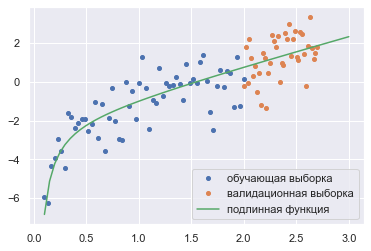
\includegraphics[width=\linewidth]{src/img/сгенерированная_выборка.png}
    \caption{Обучающая и валидационная выборки}
\end{wrapfigure}

Для заданной функции $f(h) = 1.5h - 2 - \frac{1}{2h}$ смоделируем обучающую выборку $f(h_k) + \varepsilon_k$. Точки $h_k$ выбраны равномерно на отрезке $[0.1;2]$, $к$ изменяется от $1$ до $60$. Аналогично смоделируем тестовую выборку с количеством наблюдений равным $40$. В качетсве параметров нормального распределения ошибок $\varepsilon$ было выбрано: $\mu=0, \sigma = 1$. Тестовая выборка была сгенерирована только по одну сторону от обучающей, поскольку заданная функция имеет полюс первого порядка в точке $h = 0$, и, следовательно функция при приближении к этой точке быстро растет, поэтому при генерировании точек вблизи $h=0$ значения могут быть крайне большими по модулю по сравнению с обучающей выборкой.
\newpage

\subsection{Метод наименьших квадратов}

Для модели простой линейной регрессии $X_k = \theta_0 + h\theta_1$ построим оценки МНК и МНМ, измерим качество, построенных моделей.

\begin{figure}[H]
    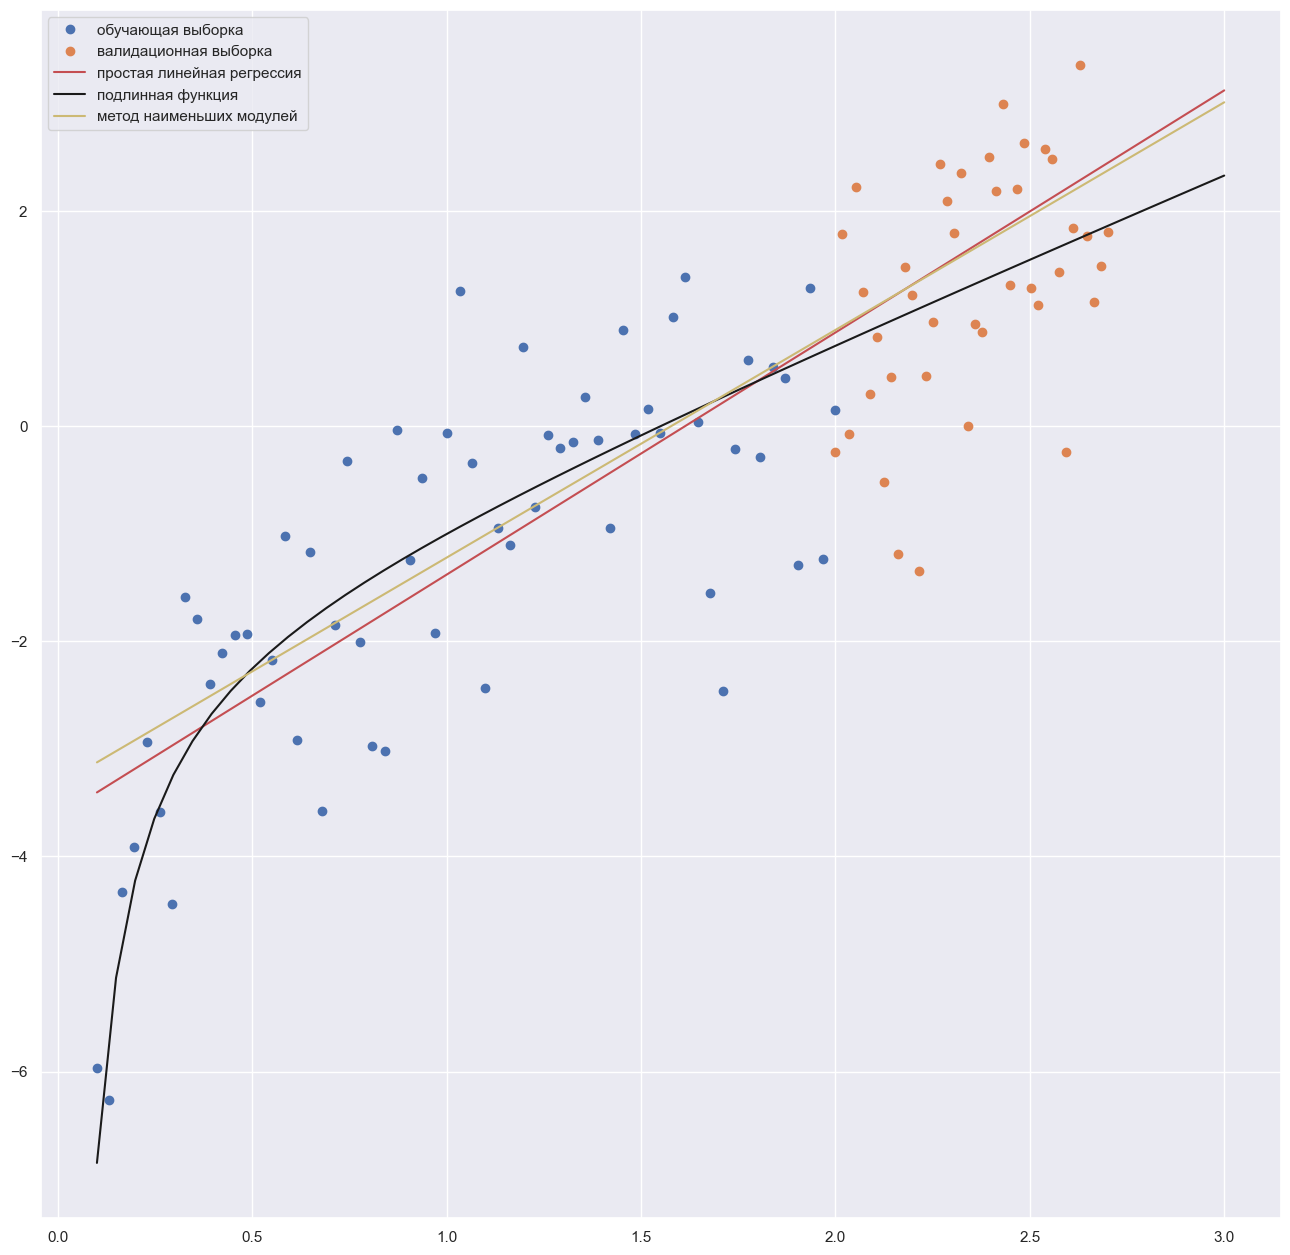
\includegraphics[width=\linewidth]{src/img/простая_линейная регрессия.png}
    \caption{Линии регрессии МНК и МНМ простой линейной регрессии}
\end{figure}

\begin{table}[H]
    \begin{center}
    \begin{tabular}{|l|c|c|}
        \hline
        & МНК & МНМ \\ \hline
        Уравнения прямых & $x = -3.63 + 2.25 h$ & $x = -3.34 + 2.12 h$ \\ \hline
        $R^2$ & $0.55$ & $0.55$ \\ \hline
        RMSE & $1.15$ & $1.16$ \\ \hline
        $\sum\limits_i \varepsilon_i^2$ (на обуч. выборке) & $78.87$ & $80.58$ \\ \hline
        $\sum\limits_i \varepsilon_i^2$ (на тест. выборке) & $44.22$ & $43.63$ \\ \hline
    \end{tabular}
    \caption{Сравнение моделей МНК и МНМ}
    \end{center}
\end{table}


\paragraph{Некоторые измерения над моделью с МНК.\\}
Оценка ковариационной матрицы:
$$ \hat{K} = 
\begin{pmatrix}
    0.10 & -0.08\\
    -0.08 & 0.08
\end{pmatrix}
$$
След оценки ковариационной матрицы $tr = 0.178$.

Функция логарифмического правдоподобия $l = -94.88$; информационный критерий Акаике $AIC = 0.39$; скорректированный (для малых выборок) $AIC_c = 0.6$; критерий Шварца $BIC = 197.95$.

Гипотеза, что $\forall i~\theta_i=0$ не принялась критерием Фишера на уровне значимости $\alpha = 0.05$.
Гипотеза, что $\theta_n = 0$ не принялась критерием Фишера на уровне значимости $\alpha = 0.05$.

Для проверки мультиколлинеарности матрицы $H^T H$ был использован коэффициент инфляции дисперсии (VIF).

Для данной модели $VIF = (4.54, 1.0)$, следовательно проблема мультиколлинеарности методом VIF не обнаружена.

\begin{figure}[H]
    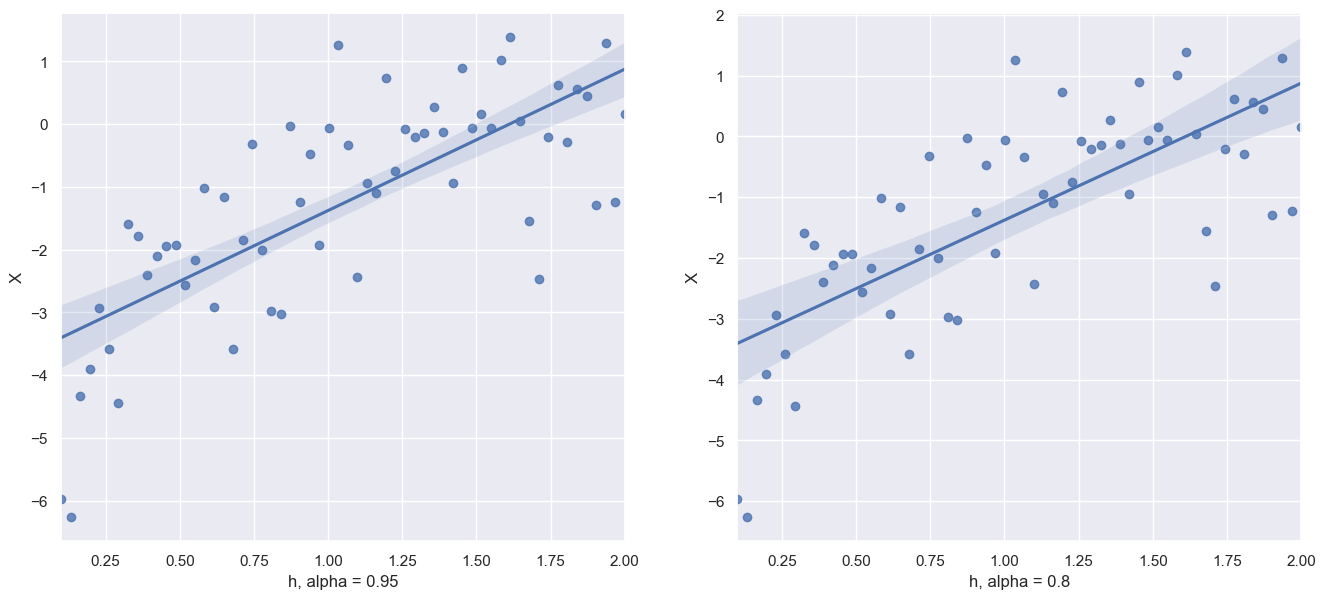
\includegraphics[width=\linewidth]{src/img/доврительные_интервалы.png}
    \caption{Доверительные интервалы для $X$ с надежностью 0.8 и 0.95}
\end{figure}


\paragraph{Анализ остатков.\\}
\begin{wrapfigure}{r}{0.3\linewidth}
    \vspace{-2ex}
    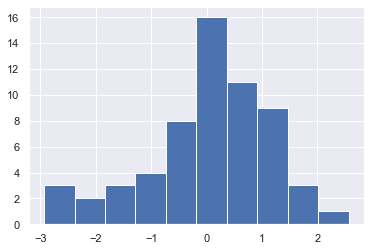
\includegraphics[width=\linewidth]{src/img/гистограмма_ошибок_1.png}
    \caption{Гистограмма ошибок}
\end{wrapfigure}

Критерий Шапиро-Уилка: $T = 0.98, pvalue = 0.29$.\\
Гипотезу о нормальном распределении ошибок на уровне значимости $0.05$ не удается принять.\\

Значение статистики Дарбина-Уотсона $ = 1.7$.\\
Выборочный коэффициент корреляции $r = 0.15$.\\
Гопотеза о некоррелированности принимается.\\

Критерий Бройша-Пагана: $(T_1 = 2.08, pvalue_1 = 0.15), (T_2 = 2.08, pvalue_2 = 0.15)$.\\
Гипотеза о гетероскедастичности принимается на уровне значимости $0.05$.\\

\begin{figure}[H]
    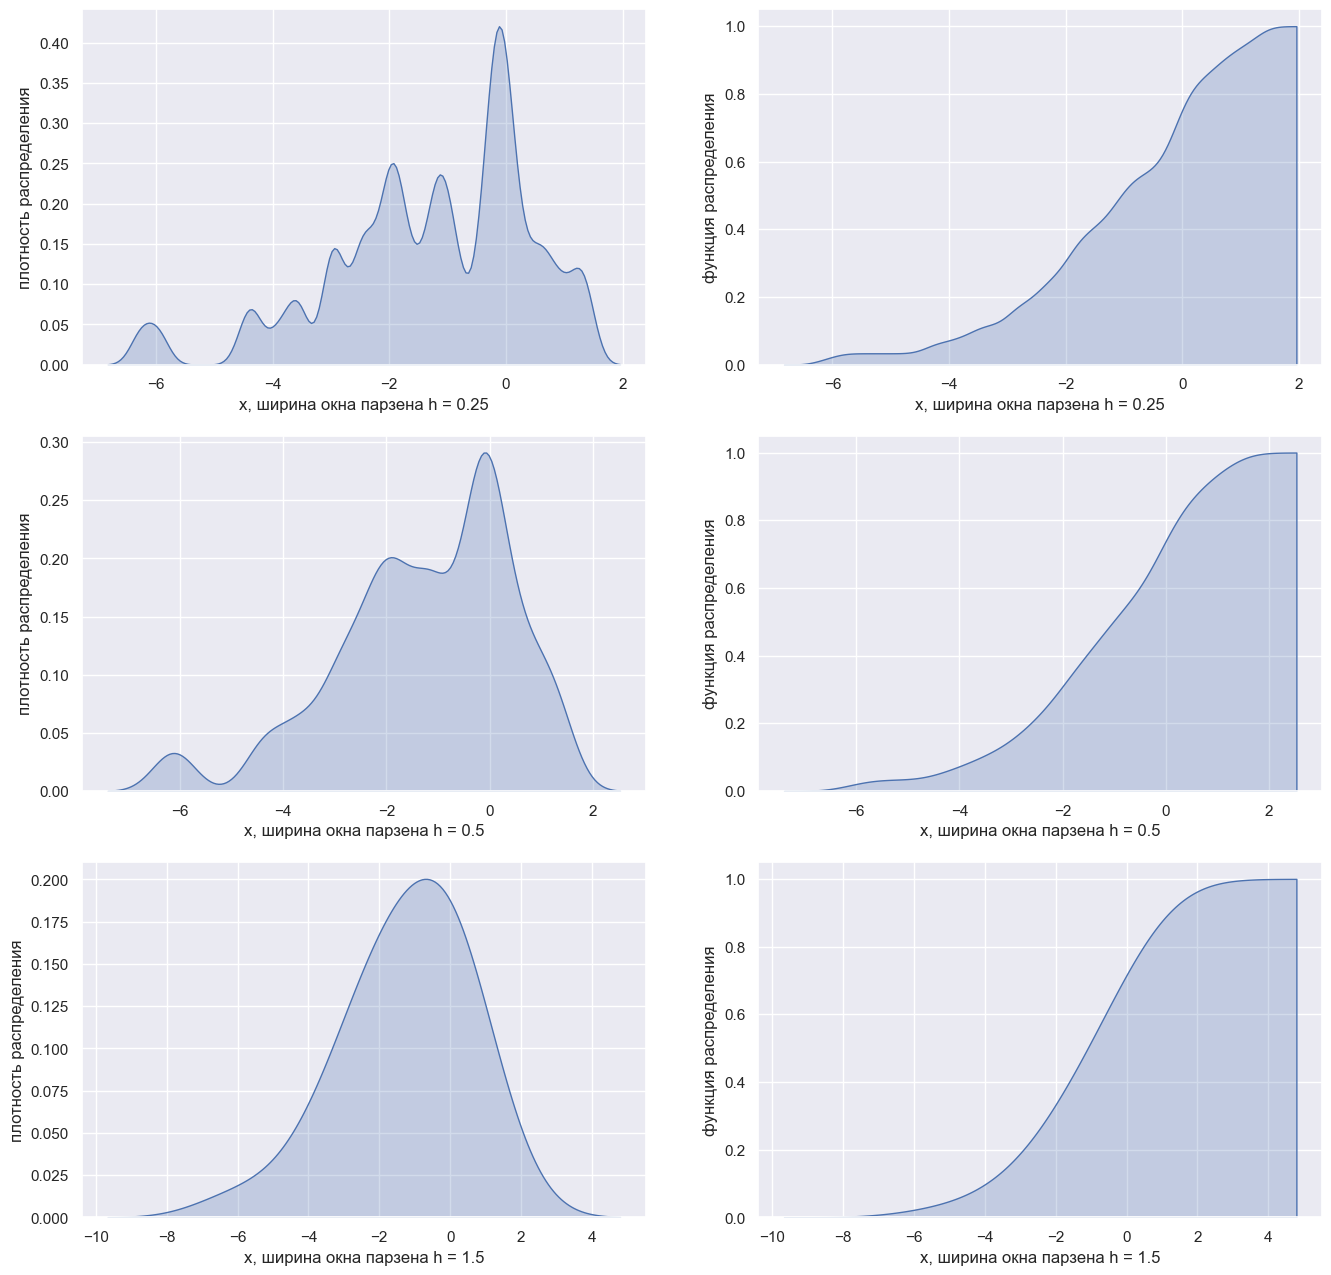
\includegraphics[width=\linewidth]{src/img/ядерные_оценки.png}
    \caption{Ядерные оценки плотности и распределения вероятности}
\end{figure}


\paragraph{Промежуточные итоги.\\}

В данной части работы было построено 2 модели простой линейной регрессии. В первой модели была использована квадратичная функция потерь, во второй был использован модуль ошибки в качестве функции потерь. Значения коэффициентов оказались близкими. Коэффициенты детерминации отличаются в 7-м знаке после запятой. При этом значение суммы квадратов отклонений на обучающей выборке немного лучше у МНК, чем у МНМ, однако на тестовой выборке наоборот. Поскольку мощность выборки не велика (60 наблюдений), был использован скорректированный критерий Акаике, который используется при малых выборках, когда число наблюдений к числу параметров меньше 40. Также были проверены гипотезы: о равенстве нулю всех параметров, о равенстве нулю последнего параметра (обе гипотезы отверглись критерием Фишера на $\alpha = 0.05$), о нормальном распределении (отверглась критерием Шапиро-Уилка на $\alpha = 0.05$), о автокорреляции (отвергалась критерием Дарбина-Уотсона), о гетероскедастичности (принялась критерием Бройша-Пагана на $\alpha = 0.05$). Построил графики ядерных оценок плотности вероятности и распределения вероятностей для разных широт окна Парзена, чем больше ширина окна, тем график более гладкий. В качестве ядра было использовано гауссово ядро.



\subsection{Полиномиальная регрессия}

Рассмотрим 6 моделей полиномиальной регрессии:
\begin{table}[H]
    \begin{center}
        \resizebox{\textwidth}{!}{
            \begin{tabular}{|p{4cm}|c|c|c|c|c|c|}
                \hline
                Количество параметров у модели (без учета $\theta_0$): & $p=1$ & $p=2$ & $p=3$ & $p=4$ & $p=5$ & $p=6$ \\ \hline
                Алгебраический вид:
                & $X = \sum\limits_{i=0}^1 \theta_i h^i$
                & $X = \sum\limits_{i=-1}^1 \theta_i h^i$
                & $X = \sum\limits_{i=-1}^2 \theta_i h^i$
                & $X = \sum\limits_{i=-1}^3 \theta_i h^i$
                & $X = \sum\limits_{i=-1}^4 \theta_i h^i$
                & $X = \sum\limits_{i=-1}^5 \theta_i h^i$ \\ \hline
            \end{tabular}
        }
        \caption{Определение моделей}
    \end{center}
\end{table}

\begin{wrapfigure}{r}{0.4\linewidth}
    \vspace{-2ex}
    \begin{minipage}[H]{0.47\linewidth}
        \center{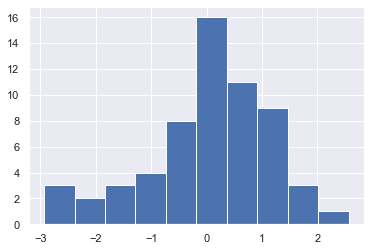
\includegraphics[width=1\linewidth]{src/img/гистограмма_ошибок_1.png}} $p=1$ \\
    \end{minipage}
    \hfill
    \begin{minipage}[H]{0.47\linewidth}
        \center{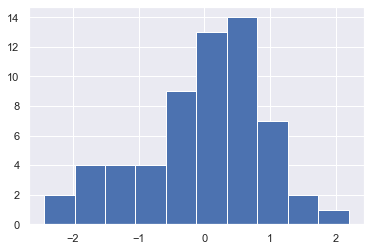
\includegraphics[width=1\linewidth]{src/img/гистограмма_ошибок_2.png}} $p=2$ \\
    \end{minipage}
    \vfill
    \begin{minipage}[H]{0.47\linewidth}
        \center{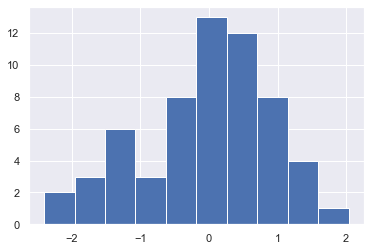
\includegraphics[width=1\linewidth]{src/img/гистограмма_ошибок_3.png}} $p=3$ \\
    \end{minipage}
    \hfill
    \begin{minipage}[H]{0.47\linewidth}
        \center{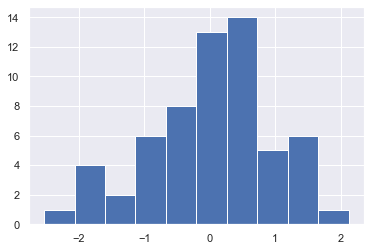
\includegraphics[width=1\linewidth]{src/img/гистограмма_ошибок_4.png}} $p=4$ \\
    \end{minipage}
    \vfill
    \begin{minipage}[H]{0.47\linewidth}
        \center{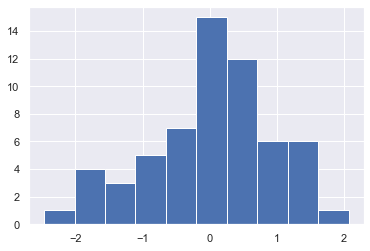
\includegraphics[width=1\linewidth]{src/img/гистограмма_ошибок_5.png}} $p=5$ \\
    \end{minipage}
    \hfill
    \begin{minipage}[H]{0.47\linewidth}
        \center{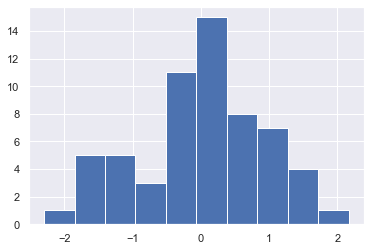
\includegraphics[width=1\linewidth]{src/img/гистограмма_ошибок_6.png}} $p=6$ \\
    \end{minipage}
    \caption{Гистограммы ошибок моделей полиномиальных регрессий}
    \label{poly_hist_errors}
\end{wrapfigure}

Заметим, что модель, соответствующая $p=1$, представляет собой модель простой линейной регрессии, рассмотренной на предыдущем шаге. В данной части она включена для наглядности сравнения с полиномиальными моделями с бОльшим числом параметров.

Обучив данные модели, были получены следующие МНК-оценки параметров:\\
Модель 1: [$-3.63$, $2.25$];\\
Модель 2: [$-1.51$, $-0.52$, $1.05$];\\
Модель 3: [$-2.76$, $-0.37$, $3.13$, $-0.8$3];\\
Модель 4: [$-0.2$, $-0.60$, $-3.94$, $5.62$, $-1.81$];\\
Модель 5: [$1.3$, $-0.71$, $-9.77$, $14.36$, $-7.24$, $1.18$];\\
Модель 6: [$-7.78$, $-0.14$, $36.02$, $-83.64$, $91.56$,\\
    $-45.23$, $8.18$].\\\newline


%\begin{table}[H]
%        \begin{tabular}{|l|p{7cm}|}
%            \hline
%            № & МНК-оценки $\hat\theta$ \\ \hline
%            1 & [$-3.63$, $2.25$] \\ \hline
%            2 & [$-1.51$, $-0.52$, $1.05$] \\ \hline
%            3 & [$-2.76$, $-0.37$, $3.13$, $-0.8$3] \\ \hline
%            4 & [$-0.2$, $-0.60$, $-3.94$, $5.62$, $-1.81$] \\ \hline
%            5 & [$1.3$, $-0.71$, $-9.77$, $14.36$, $-7.24$, $1.18$] \\ \hline
%            6 & [$-7.78$, $-0.14$, $36.02$, $-83.64$, $91.56$, $-45.23$, $8.18$] \\ \hline
%        \end{tabular}
%\end{table}


Сводная таблица с гипотезами и метриками качества моделей:
\begin{table}[H]
    \begin{center}
        %\resizebox{\textwidth}{!}{
            \begin{tabular}{|l|c|c|c|c|c|c|}
                \hline
                Номер модели & $1$ & $2$ & $3$ & $4$ & $5$ & $6$ \\ \hline
                Ср. кв. погрешность МНК-оценки & 1.15 & 0.96 & 0.95 & 0.94 & 0.93 & 0.92 \\ \hline
                Гипотеза $\theta_p = 0$ (по Фишеру) & - & - & - & - & - & + \\ \hline
                Гипотеза $\forall i~\theta_i = 0$ (по Фишеру) & - & - & - & - & - & + \\ \hline
                MSE (обуч. выборка) & $78.87$ & $55.49$ & $54.06$ & $52.47$ & $52.31$ & $52.8$ \\ \hline
                MSE (тест. выборка) & $44.22$ & $54.85$ & $145.1$ & $794.14$ & $216.31$ & $16591.33$ \\ \hline
                мультиколлинеарность матрицы $H^T H$ & - & + & + & + & + & + \\ \hline
                MSE ridge (обуч. выборка) & - & $55.5$ & $54.82$ & $53.26$ & $52.74$ & $52.8$ \\ \hline
                MSE ridge (тест. выборка) & - & $56.54$ & $76.21$ & $264.88$ & $793.6$ & $1195.54$ \\ \hline
                $tr \hat K$ & $0.18$ & $0.39$ & $4.91$ & $66.94$ & $978.41$ & $14265.62$ \\ \hline
                $R^2$ & $0.55$ & $0.68$ & $0.69$ & $0.7$ & $0.7$ & $0.71$ \\ \hline
                Гипотеза о нормальном распределении ошибок & - & - & - & - & - & - \\ \hline
                Гипотеза об автокорреляции & + & - & - & - & - & - \\ \hline
                Гипотеза о гетероскедастичности & + & + & + & + & + & + \\ \hline
            \end{tabular}
        %}
        \caption{Сводная таблица полиномиальных регрессий}
        \label{poly_table}
    \end{center}
\end{table}

\begin{figure}[H]
    \begin{minipage}[H]{0.5\linewidth}
        \center{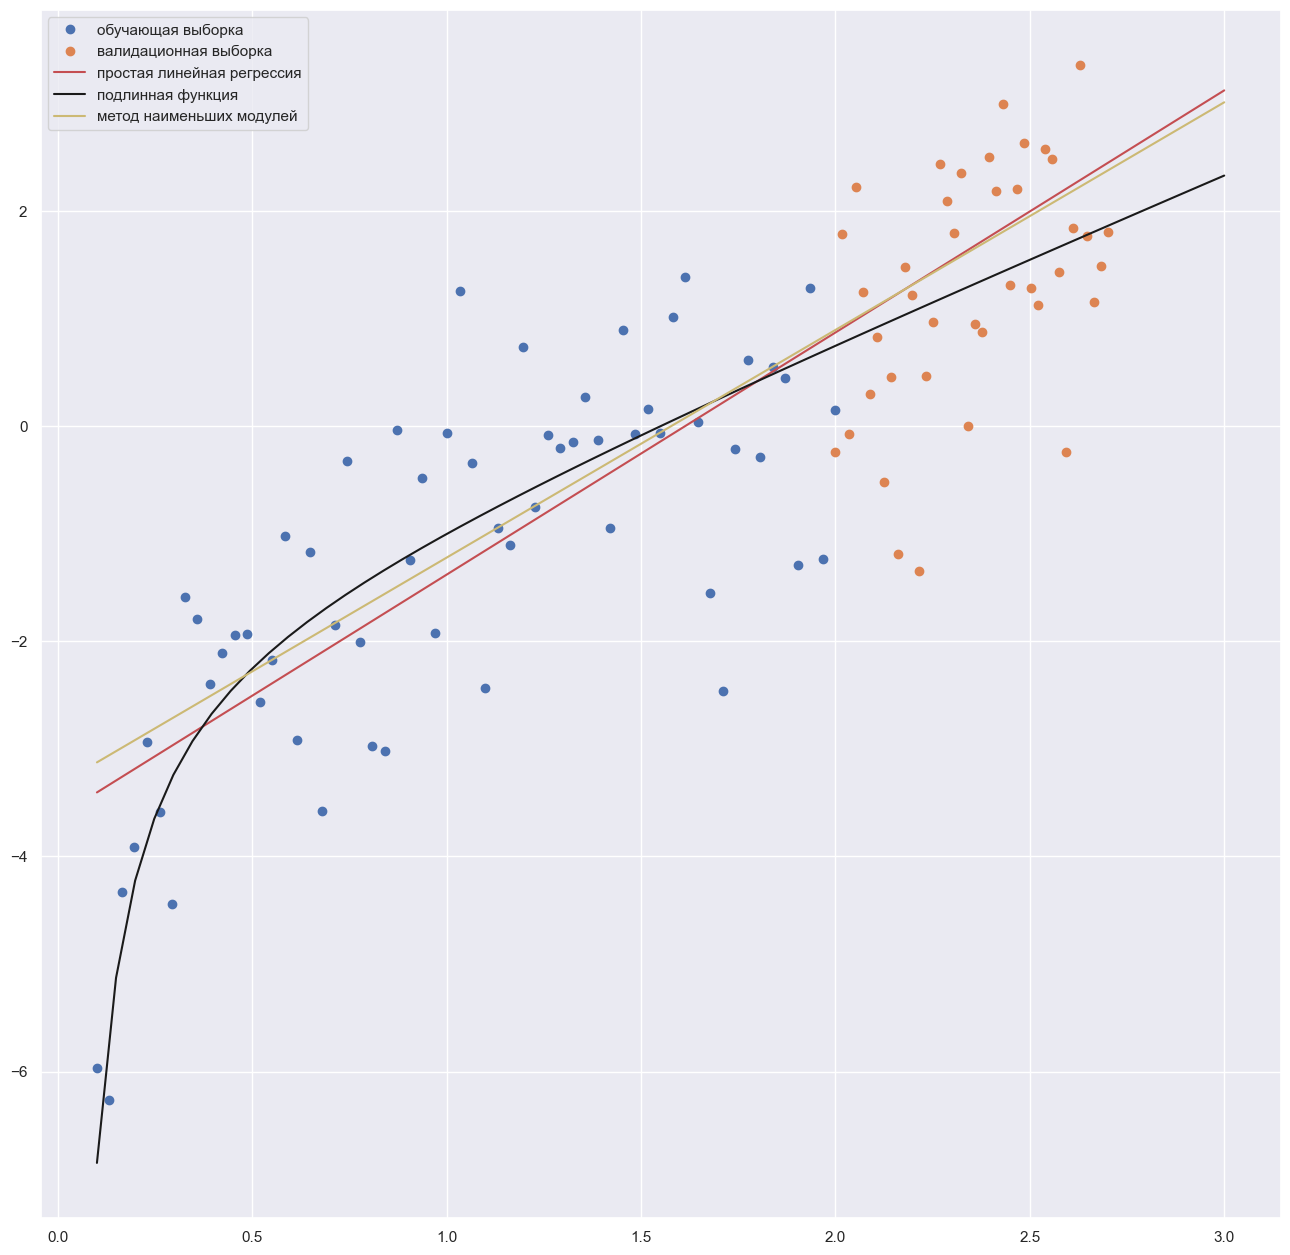
\includegraphics[width=1\linewidth]{src/img/простая_линейная регрессия.png}} $p=1$ \\
    \end{minipage}
    \hfill
    \begin{minipage}[H]{0.5\linewidth}
        \center{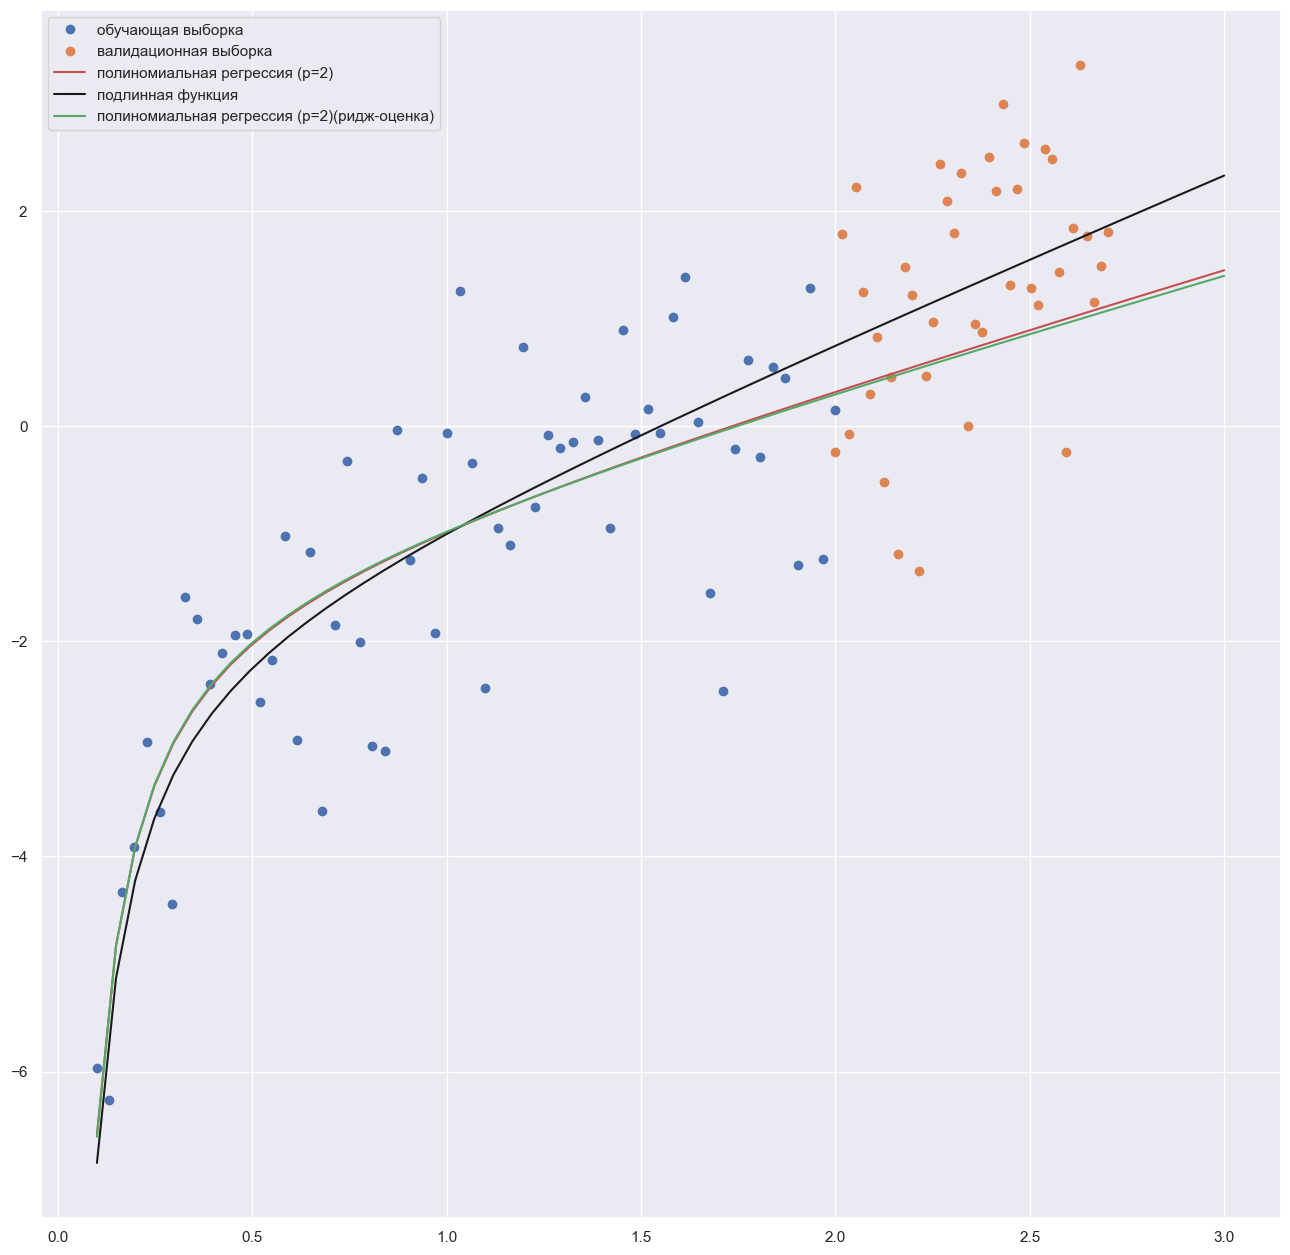
\includegraphics[width=1\linewidth]{src/img/полиномиальная_регрессия_p2.png}} $p=2$ \\
    \end{minipage}
    \vfill
    \begin{minipage}[H]{0.5\linewidth}
        \center{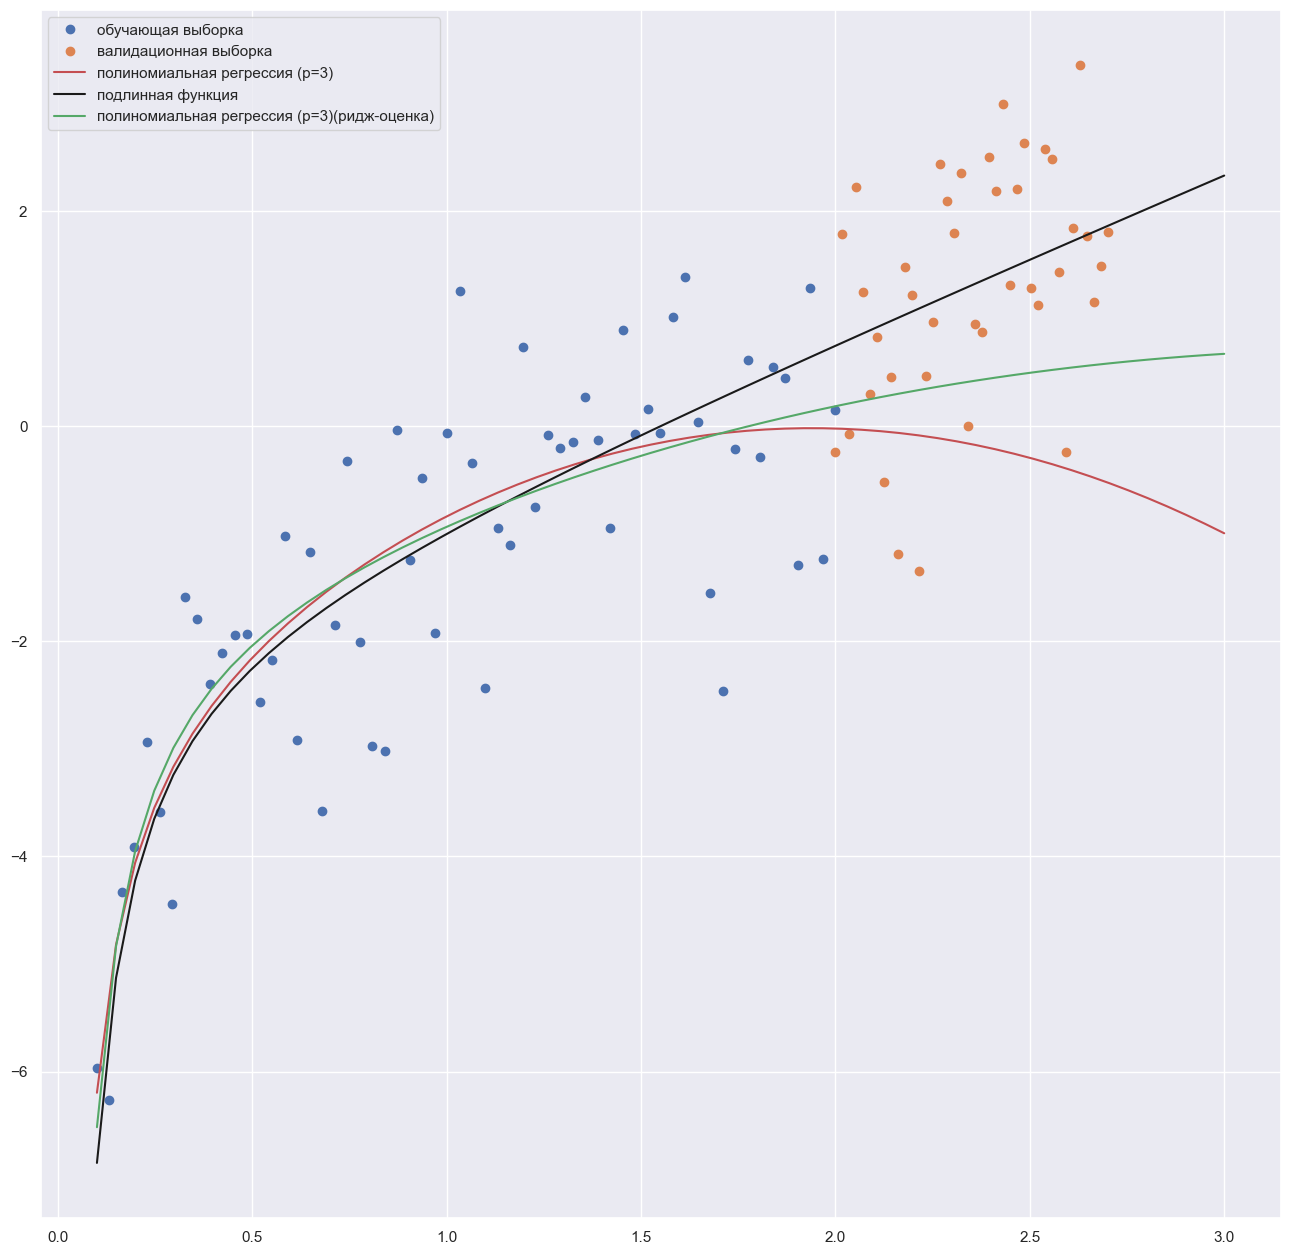
\includegraphics[width=1\linewidth]{src/img/полиномиальная_регрессия_p3.png}} $p=3$ \\
    \end{minipage}
    \hfill
    \begin{minipage}[H]{0.5\linewidth}
        \center{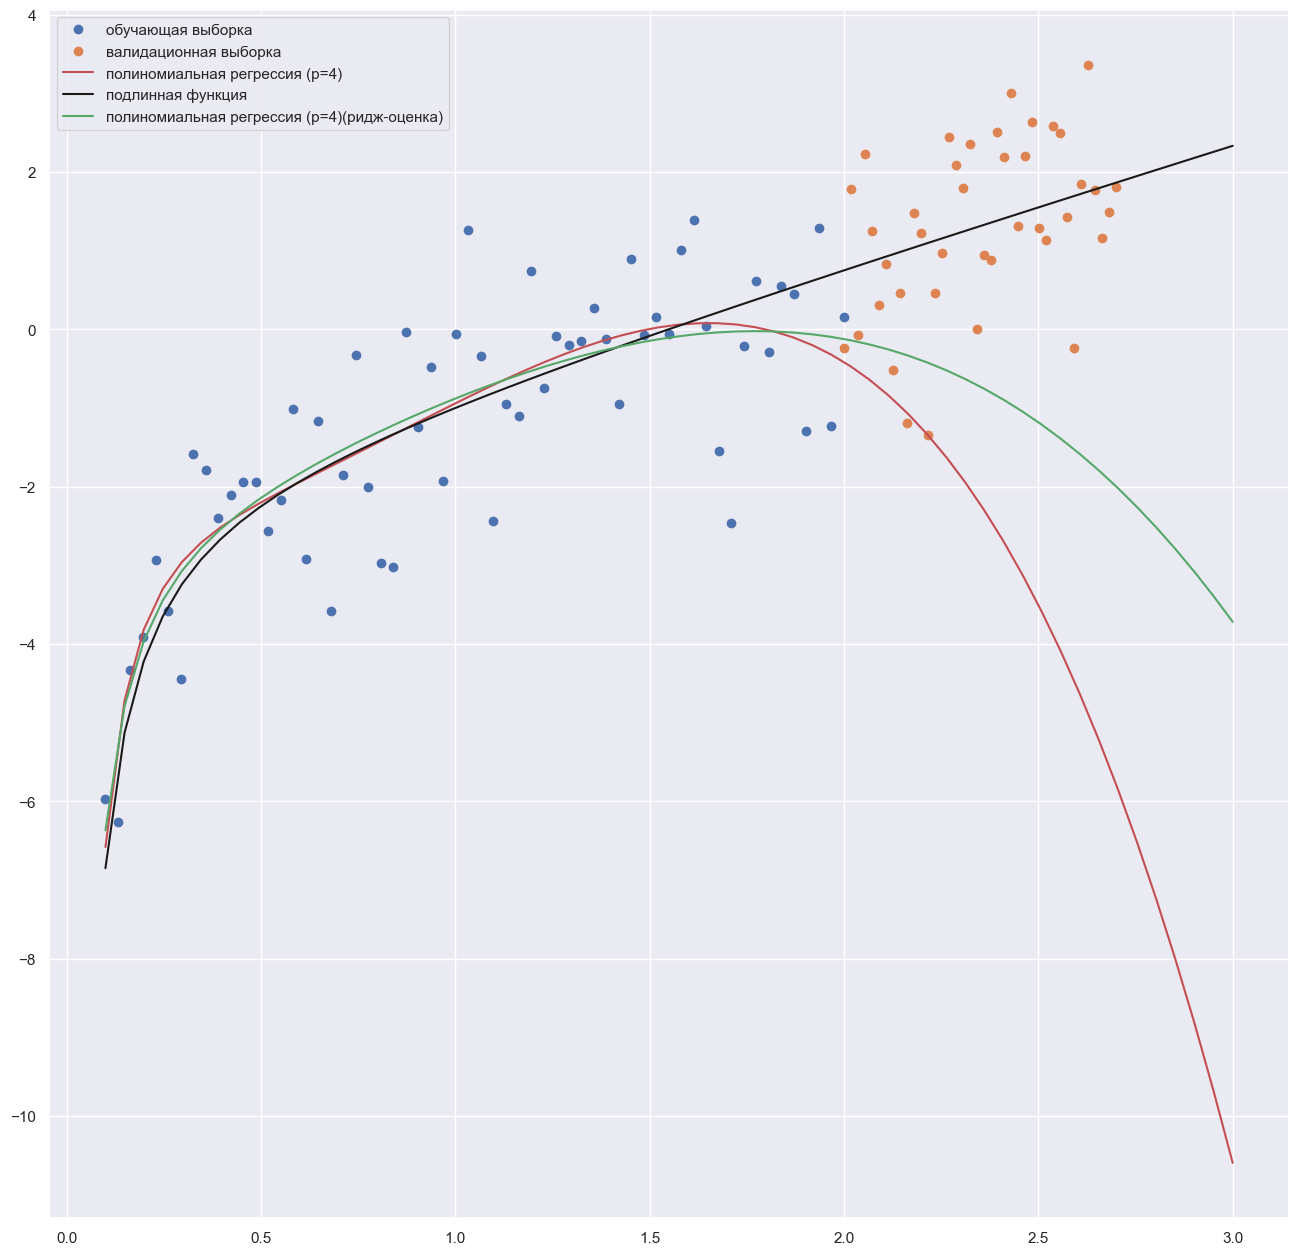
\includegraphics[width=1\linewidth]{src/img/полиномиальная_регрессия_p4.png}} $p=4$ \\
    \end{minipage}
    \vfill
    \begin{minipage}[H]{0.5\linewidth}
        \center{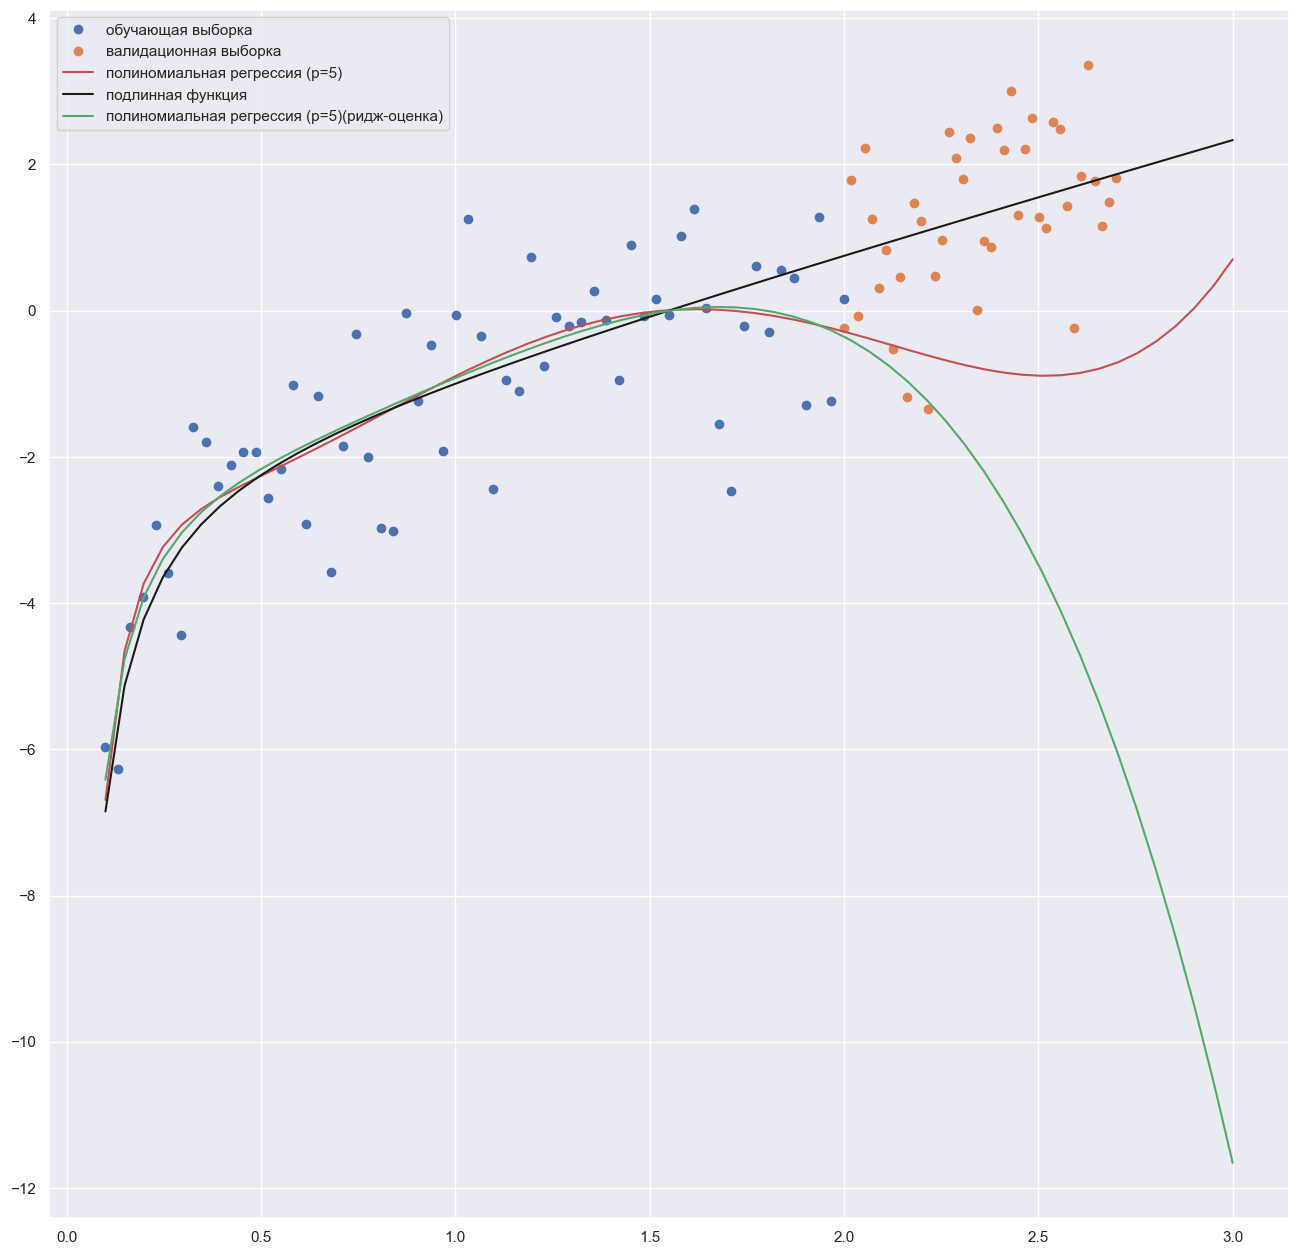
\includegraphics[width=1\linewidth]{src/img/полиномиальная_регрессия_p5.png}} $p=5$ \\
    \end{minipage}
    \hfill
    \begin{minipage}[H]{0.5\linewidth}
        \center{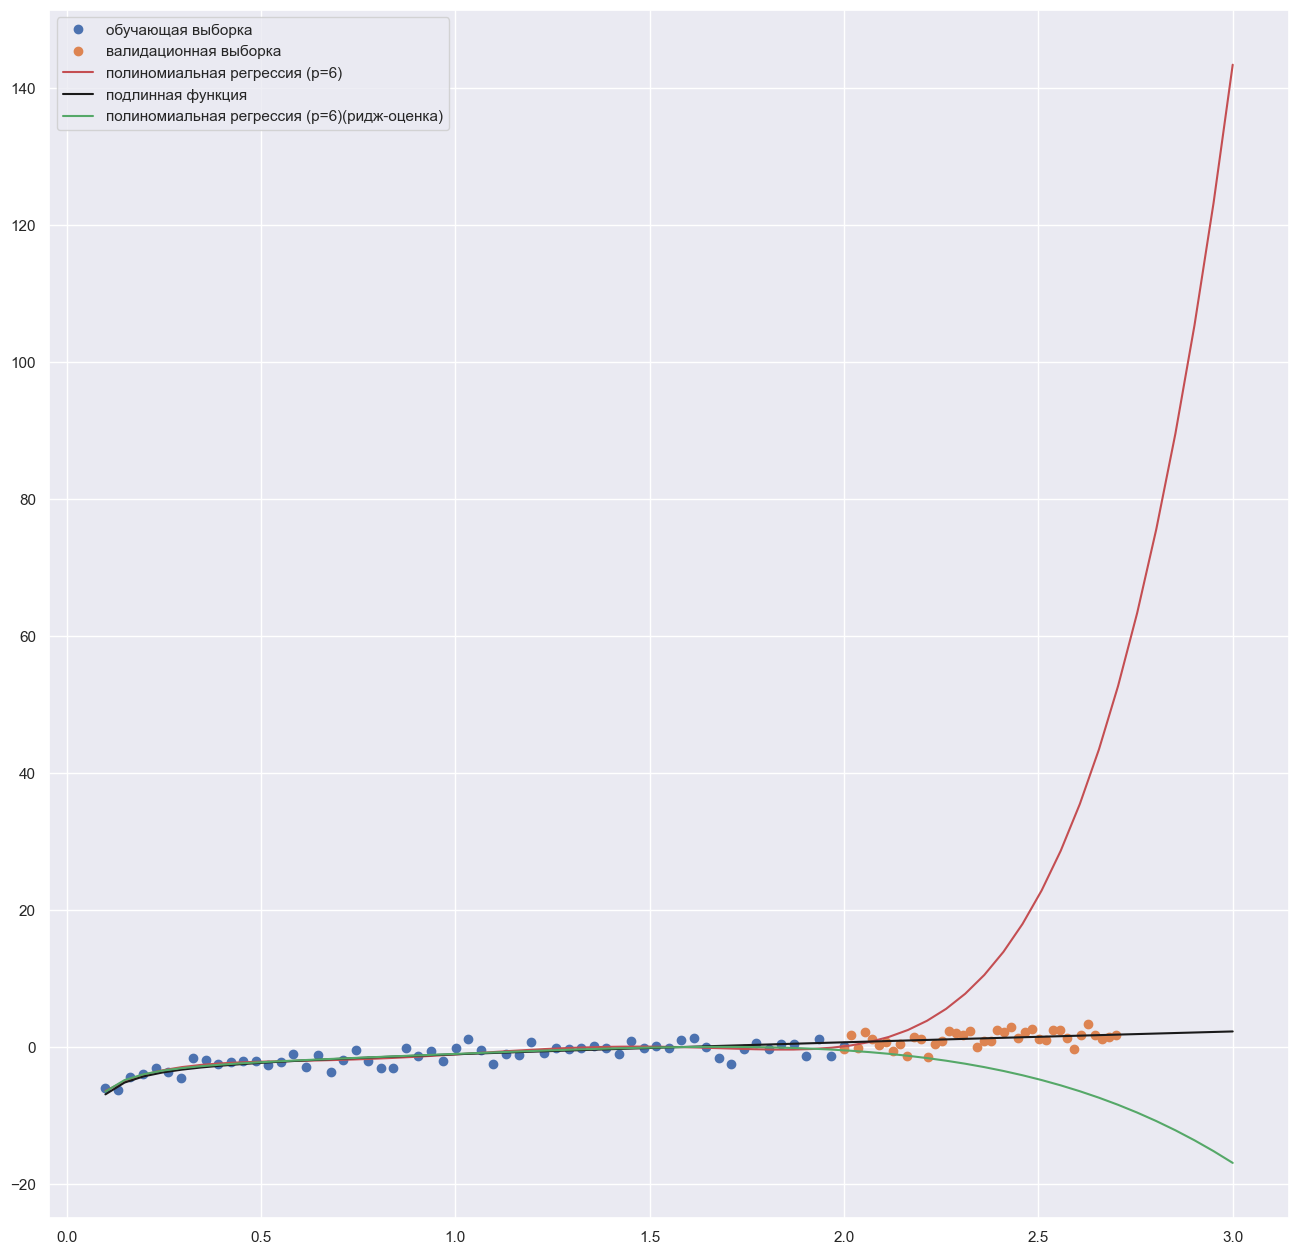
\includegraphics[width=1\linewidth]{src/img/полиномиальная_регрессия_p6.png}} $p=6$ \\
    \end{minipage}
    \caption{Линии регрессий}
    \label{poly_lines}
\end{figure}


\paragraph{Промежуточные итоги.\\}
В данной части было проанализированно 6 моделей полиномиальной регрессии. По данным таблицы \ref{poly_table} можно заметить классический пример эффекта переобучения: MSE на обучающей выборке с ростом числа параметров незначительно уменьшается, при этом MSE на валидационной выборке быстро растет. Во всех моделях, кроме первой матрица $H^T H$ мультиколлинеарна, для таких моделей были построены ridge-оценки. На обучающей выборке MSE-оценки ridge моделей примерно совпадают с MSE-оценками МНК моделей, однако на валидационной выборке данные модели имеют существенно более низкие показатели. Следует заметить, что для пятой модели MSE ridge хуже MSE МНК, это можно легко объяснить по графику \ref{poly_lines} при $p=5$: ridge-оценка привела к уменьшению значения параметра при старшей степени, что повлекло к развороту многочлена вниз (зеленая кривая), в то время расстояние от кривой, соответствующей МНК-оценке, до валидационной выборки многократно меньше.

Начиная с $p=3$ $tr K$, MSE, MSE ridge на тестовой выборке начинают ухудшаться. $R^2$ практически не изменяется. Следовательно, оптимальным значением для параметра полиномиальной регрессии является $p=2$. Однако, судя по графикам на рисунке \ref{poly_lines} для $p=2$ модели не хватило данных для обучения, поскольку кривая с приблизительно $h=1.5$ начинает отклоняться вниз от искомой зависимости, а простая линейная регрессия не смогла описать зависимость данных около $h=0$ и также отклоняется от искомой зависимости, но уже в большую сторону. Возможно, имеет смысл скорректировать параметр при $h$ у модели c $p=2$ и взять его как среднее арифметическое параметров при $h$ у моделей $p=1$ и $p=2$.

Гипотезу о гетероскедастичности не удалось отвергнуть ни у одной модели. Гипотеза о нормальном распределении ошибок была отвергнута во всех моделях. Гипотеза об автокорреляции была отвергнута во всех моделях, кроме первой.
\newpage


\subsection{Регрессия для наблюдений с выбросами}

Смоделируем распределение Тьюки. Для этого сгенерируем 3 массива случайных чисел: $u, v, w$, выберем долю выбросов $\delta=0.08$ и силу выбросов $sigma_1 = 10\sigma$.
\begin{itemize}
    \item $u=(u_1,\ldots,u_{60}),~~u_i \sim \mathcal{N}(0,\sigma^2)$ -- обычные наблюдения;
    \item $v=(v_1,\ldots,v_{60}),~~v_i \sim \mathcal{N}(0,(10\sigma)^2)$ -- выбросы;
    \item $w=(w_1,\ldots,w_{60}),~~w_i \sim \mathcal{R}(0,1)$ -- вектор вероятностей.
\end{itemize}

Сформируем из сгенерированных массивов выборку по следующему алгоритму:
\begin{minted}[fontsize=\footnotesize, linenos, breaklines, breakafter=d, frame=lines]{python}
X = [ ]
for i in range(len(u)):
    if w[i] < delta:
        X.append(f(h[i]) + u[i])
    else:
        X.append(f(h[i]) + v[i])
\end{minted}

Аналогично сгенерируем тестовую выборку.\\
Результат моделирования (график приведен в логарифмическом масштабе по вертикальной оси); также построим модели простой линейной модели для МНК и МНМ на данных с выбросами:

\begin{figure}[H]
    \centering
    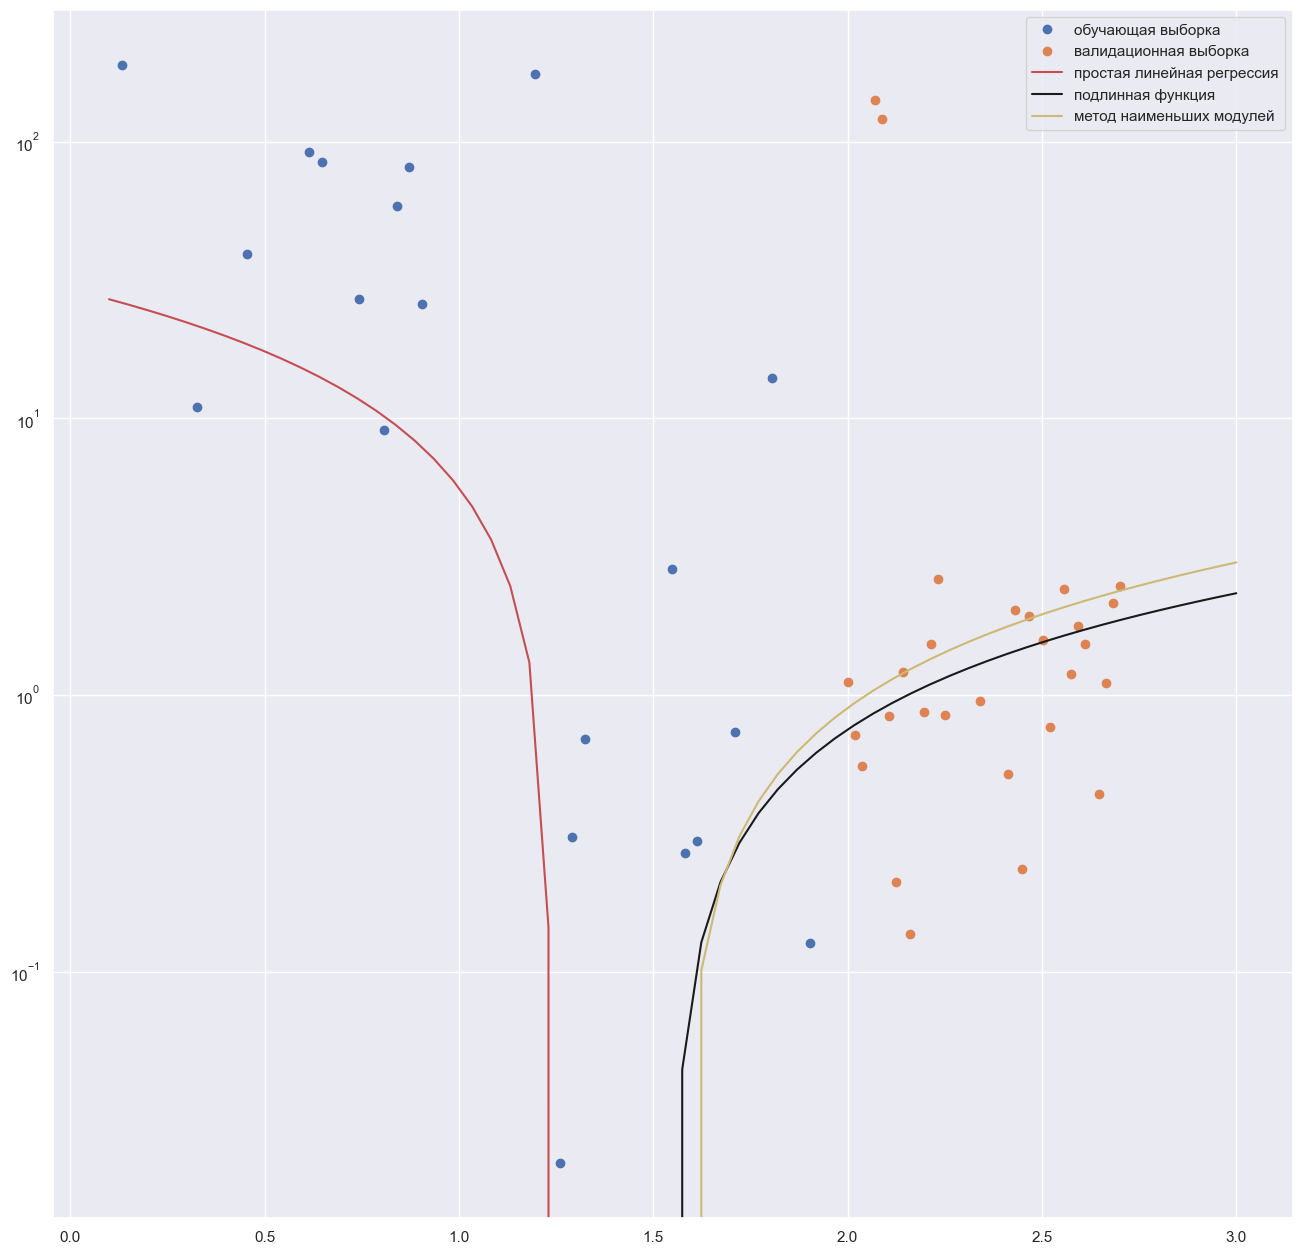
\includegraphics[width=0.5\linewidth]{src/img/простая_линейная регрессия_с_выбросами.png}
    \caption{Линии регрессий для наблюдений с выбросами}
\end{figure}

\begin{table}[H]
    \begin{center}
        \begin{tabular}{|l|c|c|}
            \hline
            & МНК & МНМ \\ \hline
            Уравнения прямых & $x = 29.34 - 23.73 h$ & $x = -3.36 + 2.11 h$ \\ \hline
            $R^2$ & $0.07$ & $0.07$ \\ \hline
            RMSE & $47.9$ & $50.33$ \\ \hline
            $\sum\limits_i \varepsilon_i^2$ (на обуч. выборке) & $137649.99$ & $151957.64$ \\ \hline
            $\sum\limits_i \varepsilon_i^2$ (на тест. выборке) & $96192.08$ & $73400.67$ \\ \hline
        \end{tabular}
        \caption{Сравнение моделей МНК и МНМ на данных с выбросами}
    \end{center}
\end{table}

\paragraph{Некоторые измерения над моделью с МНК.\\}
Оценка ковариационной матрицы:
$$ \hat{K} = 
\begin{pmatrix}
    182.92 & -135.87\\
    -135.87 & 129.4
\end{pmatrix}
$$
След оценки ковариационной матрицы $tr = 312.32$.

Функция логарифмического правдоподобия $l = -318.82$; информационный критерий Акаике $AIC = 7.86$; скорректированный (для малых выборок) $AIC_c = 8.07$; критерий Шварца $BIC = 645.83$.

Гипотеза, что $\forall i~\theta_i=0$ принялась критерием Фишера на уровне значимости $\alpha = 0.005$.
Гипотеза, что $\theta_n = 0$ принялась критерием Фишера на уровне значимости $\alpha = 0.005$.

$VIF = (4.54, 1.0)$, следовательно проблема мультиколлинеарности методом VIF не обнаружена.


\paragraph{Анализ остатков.\\}
\begin{wrapfigure}{r}{0.3\linewidth}
    \vspace{-2ex}
    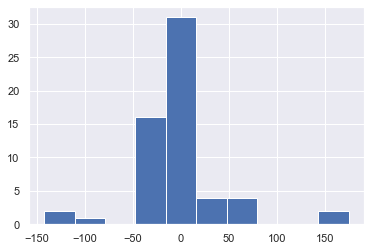
\includegraphics[width=\linewidth]{src/img/гистограмма_ошибок_наблюдения_с_выбросами.png}
    \caption{Гистограмма ошибок для наблюдений с выбросами}
\end{wrapfigure}

Критерий Шапиро-Уилка: $T = 0.82$, $pvalue = 3.81\cdot10^{-7}$.\\
Распределение ошибок нормальное на уровне значимости 0.05.\\

Значение статистики Дарбина-Уотсона $T = 1.99$.\\
Выборочный коэффициент корреляции $r = 0.003$.\\
Гипотеза о некоррелированности принимается.\\

Критерий Бройша-Пагана: $(T_1 = 2.11, pvalue_1 = 0.35), (T_2 = 1.04, pvalue_2 = 0.36)$.\\
Гипотеза о гетероскедастичности принимается на уровне значимости $0.05$.\\


\paragraph{Отбраковка выбросов.\\}

Отбраковку выбросов будем проводить следующим образом:
\begin{enumerate}
    \item построение регрессии Тьюки или Хьюбера;
    \item отбраковка тех значений, которые лежат более чем на $3\sigma$ от регрессионной кривой Тьюки или Хьюбера;
\end{enumerate}

\begin{wrapfigure}{r}{0.3\linewidth}
    \vspace{-2ex}
    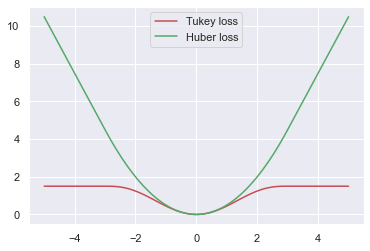
\includegraphics[width=\linewidth]{src/img/Тьюки_и_Хьюбер.png}
    \caption{Функции потерь Хьюбера и Тьюки для параметра $\delta=3$}
\end{wrapfigure}

Линейная регрессия называется регрессией Тьюки, если в качестве функции потерь взята функция потерь Тьюки:
$$
\begin{cases}
    \frac{\delta^2}{6} \cdot \left(1 - \left(1 - \left(\frac{u}{\delta} \right)^2\right)^3\right), & |u| < \delta\\
    \frac{\delta^2}{6}, & \text{иначе}
\end{cases}
$$

Также рассмотрим регрессию Хьюбера. Линейная регрессия называется регрессией Хьюбера, если в качестве функции потерь взята функция потерь Хьюбера:
$$
\begin{cases}
    \frac{u^2}{2}, & |u| < \delta\\
    \delta \cdot \left( |u| - \frac{\delta}{2} \right), & \text{иначе}
\end{cases}
$$

Построим регрессии. Регрессия Хьюбера строилась для параметра $\delta = 0.1$, регрессия Тьюки строилась для параметра $\delta = 3$.

\begin{figure}[H]
    \centering
    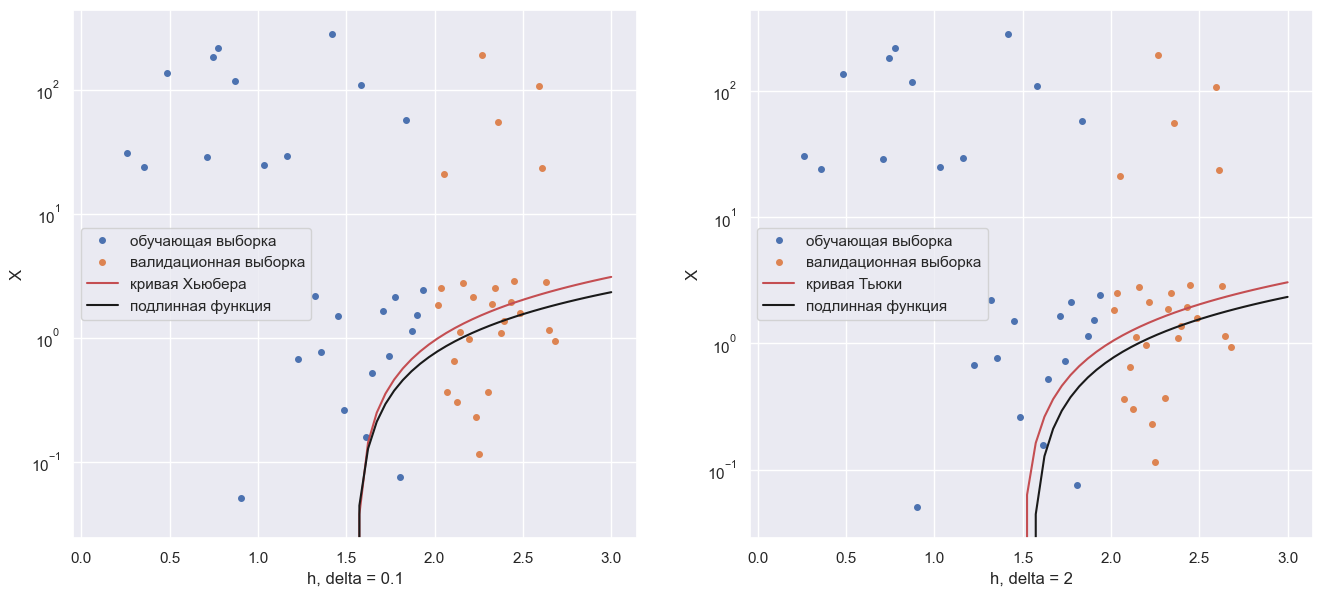
\includegraphics[width=\linewidth]{src/img/линии_Тьюки_и_Хьюбера.png}
    \caption{Линии регрессий Хьюбера и Тьюки в логарифмическом по X масштабе}
\end{figure}

Для построенных регрессий высчитаем характеристики качества:

\begin{table}[H]
    \begin{center}
        \begin{tabular}{|l|c|c|}
            \hline
            & Хьюбер & Тьюки \\ \hline
            Уравнения прямых & $x = -3.34 + 2.15 h$ & $x = -3.02 + 2.02 h$ \\ \hline
            $R^2$ & $0.55$ & $0.55$ \\ \hline
            RMSE & $1.16$ & $1.21$ \\ \hline
            $\sum\limits_i \varepsilon_i^2$ (на обуч. выборке) & $80.94$ & $87.9$ \\ \hline
            $\sum\limits_i \varepsilon_i^2$ (на тест. выборке) & $45.49$ & $46.52$ \\ \hline
        \end{tabular}
        \caption{Сравнение моделей Хьюбера и Тьюки на данных с выбросами}
    \end{center}
\end{table}

Сделаем отбраковку выбросов по построенной кривой Хьюбера и построим на получившимся наборе данных МНК и МНМ оценки:

\begin{figure}[H]
    \centering
    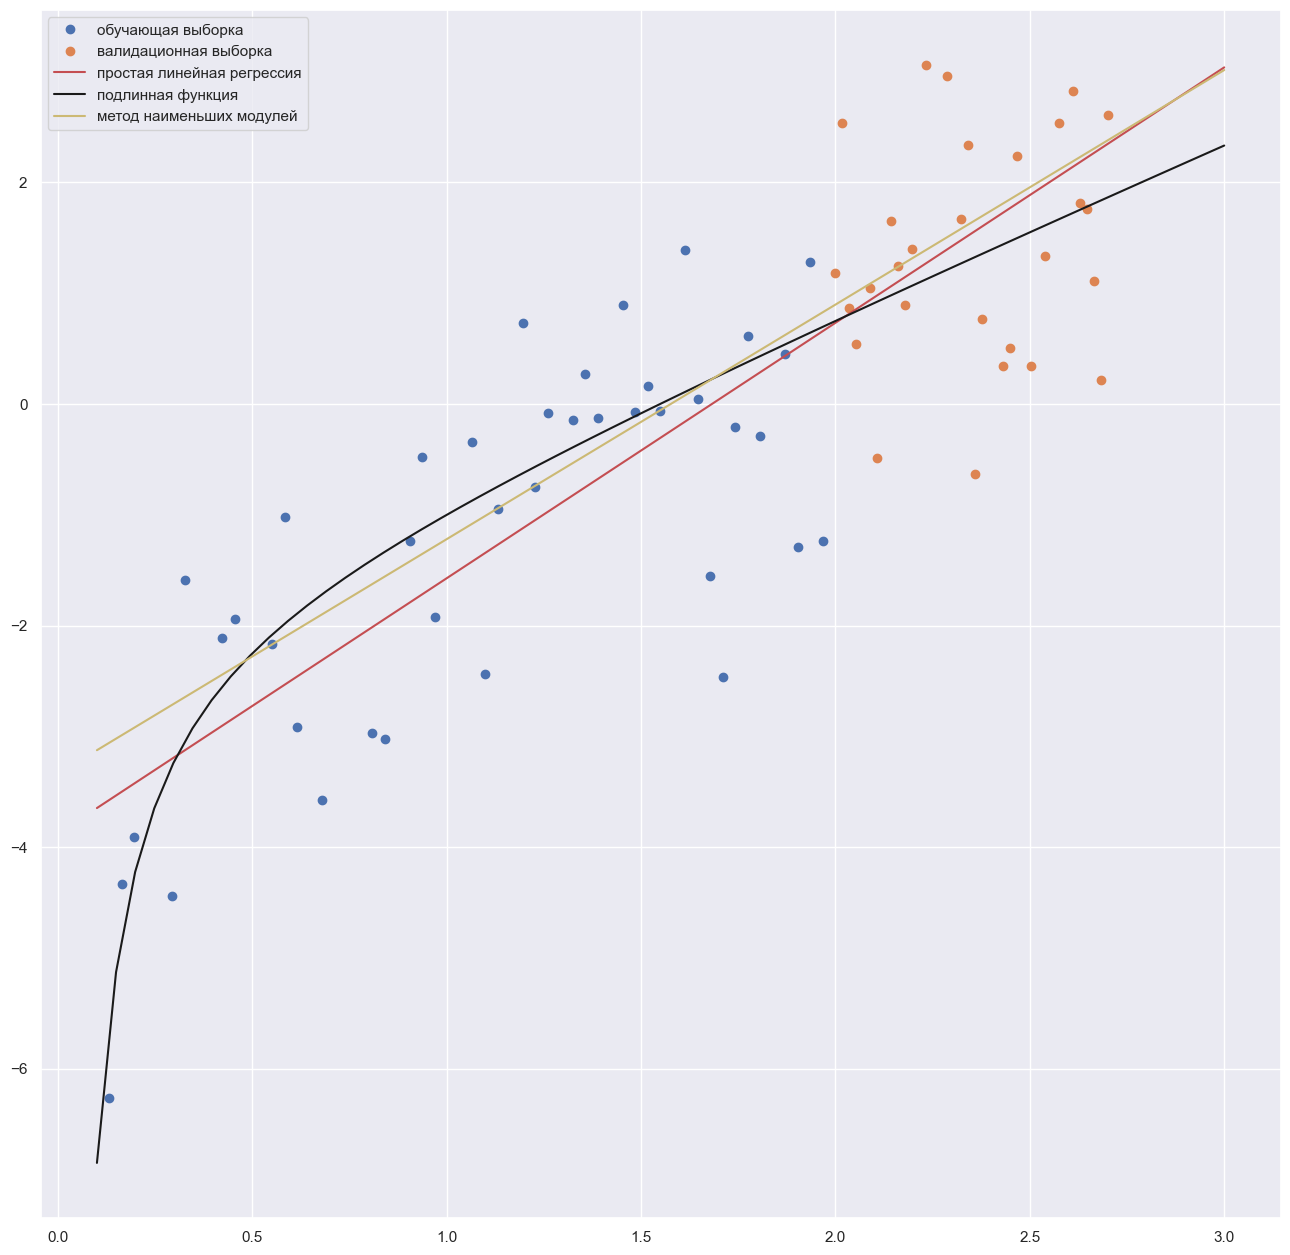
\includegraphics[width=0.5\linewidth]{src/img/данные_без_выбросов.png}
    \caption{МНК и МНМ оценки для данных, очищенных от выбросов}
\end{figure}

\begin{table}[H]
    \centering
    \begin{tabular}{|l|c|c|}
        \hline
        & МНК & МНМ \\ \hline
        Уравнения прямых & $x = -3.88 + 2.31 h$ & $x = -3.37 + 2.12 h$ \\ \hline
        $R^2$ & $0.55$ & $0.55$ \\ \hline
        RMSE & $1.14$ & $1.19$ \\ \hline
        $\sum\limits_i \varepsilon_i^2$ (на обуч. выборке) & $52.08$ & $56.77$ \\ \hline
        $\sum\limits_i \varepsilon_i^2$ (на тест. выборке) & $31.22$ & $31.54$ \\ \hline
    \end{tabular}
    \caption{Сравнение моделей МНК и МНМ на данных, очищенных от выбросов}
\end{table}


\paragraph{Некоторые измерения над моделью с МНК.\\}
Оценка ковариационной матрицы:
$$ \hat{K} = 
\begin{pmatrix}
    0.19 & -0.13\\
    -0.13 & 0.12
\end{pmatrix}
$$
След оценки ковариационной матрицы $tr = 0.3$.

Функция логарифмического правдоподобия $l = -95.39$; информационный критерий Акаике $AIC = 0.41$; скорректированный (для малых выборок) $AIC_c = 0.62$; критерий Шварца $BIC = 198.97$.

Гипотеза, что $\forall i~\theta_i=0$ не принялась критерием Фишера на уровне значимости $\alpha = 0.05$.
Гипотеза, что $\theta_n = 0$ не принялась критерием Фишера на уровне значимости $\alpha = 0.05$.

$VIF = (5.28, 1.0)$, следовательно проблема мультиколлинеарности методом VIF не обнаружена.


\paragraph{Анализ остатков.\\}
\begin{wrapfigure}{r}{0.3\linewidth}
    \vspace{-2ex}
    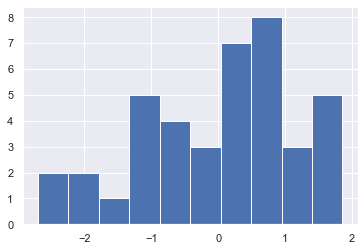
\includegraphics[width=\linewidth]{src/img/гистограмма_ошибок_без_выбросов.png}
    \caption{Гистограмма ошибок для наблюдений, очищенных от выбросов}
\end{wrapfigure}

Критерий Шапиро-Уилка: $T = 0.96$, $pvalue = 0.13$.\\
Гипотезу о нормальном распределении ошибок на уровне 0.05 не удается принять.\\

Значение статистики Дарбина-Уотсона $T = 1.35$.\\
Выборочный коэффициент корреляции $r = 0.33$.\\
Гипотеза о некоррелированности отвергается.\\

Критерий Бройша-Пагана: $(T_1 = 0.13, pvalue_1 = 0.7), (T_2 = 0.12, pvalue_2 = 0.72)$.\\
Гипотеза о гетероскедастичности принимается на уровне значимости $0.05$.


\paragraph{Промежуточные итоги.\\}

В данной части были смоделированы данные с выбросами с помощью распределения Тьюки. Для данных с выбросами были получены МНК и МНМ оценки. Качество таких моделей оказалось крайне плохим, однако по графику видно, что МНМ-оценка находится близко к подлинной функции. Были построены модели регрессии Тьюки и Хьюбера, данные модели смогли распознать выбросы и добиться приемлемого качества как на обучающей выборке, так и на валидационной. По графику с функциями потерь Хьюбера и Тьюки можно сделать выводы: функция потерь Тьюки используется при наличие больших по модулю выбросов, поскольку штраф за ошибки, по модулю больше чем $\delta$ (параметр функции Тьюки), является константой, если же известно, что доля выбросов не велика, то имеет смысл применить функцию потерь Хьюбера, для которого вне $\delta$-окрестности фактически применяется МНМ, в внутри окрестности МНК.

Отбраковка выбросов была сделана с помощью оценки Хьюбера: данные, отстающие более, чем на $3\sigma$ от кривой Хьюбера исключаются из выборки.



\subsection{Квантильная регрессия}

Смоделируем несимметричные ошибки на исходных данных, заменив $90\%$ отрицательных ошибок на их абсолютное значение. И построим МНК и МНМ оценки:
\begin{figure}[H]
    \centering
    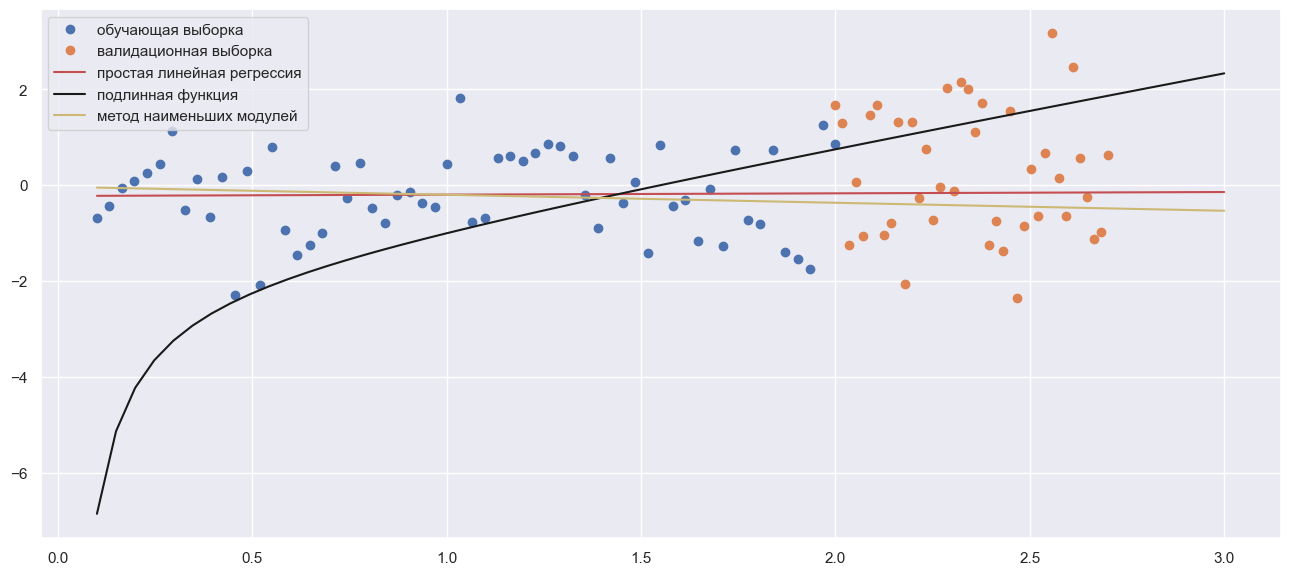
\includegraphics[width=\linewidth]{src/img/несимметричные_ошибки.png}
    \caption{МНК и МНМ оценки для данных с несимметричными ошибками}
\end{figure}

\begin{table}[H]
    \centering
    \begin{tabular}{|l|c|c|}
        \hline
        & МНК & МНМ \\ \hline
        Уравнения прямых & $x = -0.22 + 0.03 h$ & $x = -0.03 - 0.17 h$ \\ \hline
        $R^2$ & $0.0003$ & $0.0003$ \\ \hline
        RMSE & $0.86$ & $0.87$ \\ \hline
        $\sum\limits_i \varepsilon_i^2$ (на обуч. выборке) & $45.08$ & $45.79$ \\ \hline
        $\sum\limits_i \varepsilon_i^2$ (на тест. выборке) & $77.08$ & $88.66$ \\ \hline
    \end{tabular}
    \caption{Сравнение моделей МНК и МНМ на данных с несимметричными ошибками}
\end{table}

\begin{figure}[H]
    \centering
    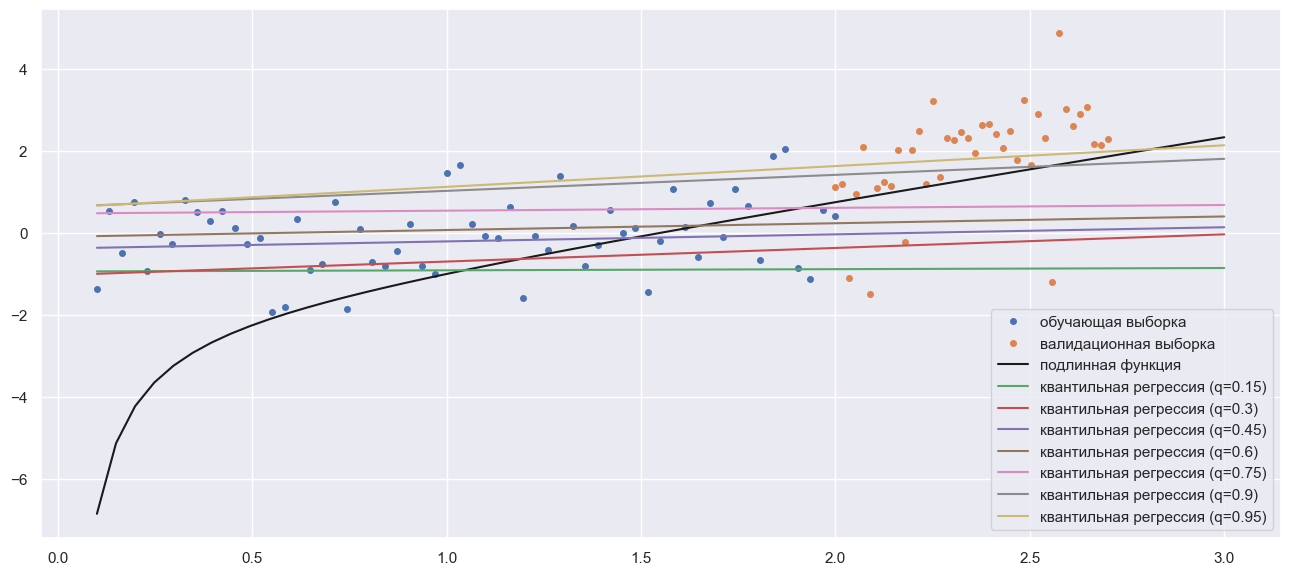
\includegraphics[width=\linewidth]{src/img/квантильная_регрессия.png}
    \caption{Квантильная регрессия для различных значений уровня квантиля}
\end{figure}

\begin{table}[H]
    \centering
    \begin{tabular}{|l|c|c|c|c|c|c|}
        \hline
        Квантиль q & 0.15 & 0.3 & 0.45 & 0.6 & 0.75 & 0.9 \\ \hline
        Pseudo $R^2$ & 0.04 & 0.011 & 0.003 & 0.0004 & 0.062 & 0.017 \\ \hline
    \end{tabular}
    \caption{Качество квантильных регрессия для разных уровней квантилей}
\end{table}

\paragraph{Промежуточные итоги.\\}
МНК и МНМ модели не смогли распознать несимметричные ошибки, судя по графику. Были построены модели квантильной регрессии для набора параметров квантилей ($0.15$, $0.3$, $0.45$, $0.6$, $0.75$, $0.9$), квантильная регрессия также не смогла распознать такие ошибки для данного набора данных, что видно по графику и по данным таблицы с pseudo $R^2$.



\section{Выводы}

В ходе работы был смоделирован набор данных по заданной функции, для него были построенны МНК и МНМ оценки, вычислены метрики качества, построены доверительные интервалы, а также был проведен анализ остатков, построены ядерные оценки.

Повысить качество модели удалось за счет применения полиномиальной регрессии, ожидаемо модель $X=\sum\limits_{i=-1}^1 \theta_i h^i$ оказалась наиболее лучшей. Всего было построенно 6 моделей полиномиальной регрессии, для каждой модели были вычислены метрики качества, проверены параметрические гипотезы, также был сделан анализ остатков для каждой модели.

Были смоделированы наблюдения с выбросами по распределению Тьюки. МНК и МНМ оценки оказались неудачными, поэтому были построены оценки Тьюки и Хьюбера, которые дали хорошие показатели качества на обучающей и тестовой выборках. На основе регрессии Хьюбера был реализован алгоритм по фильтрации выбросов. Полученные новые МНК и МНМ оценки оказались более точными, чем оценка Хьюбера.

Также была создана выборка с несимметричными ошибками. Для данного набора данных МНК и МНМ оценки не смогли восстановить искомую зависимость, при построение квантильной регрессии модели также не распознали асимметричные ошибки, при увеличении $h$ разница между прогнозным значением и ожидаемым также растет.




\section{Список источников}

\end{document}}